\documentclass[tikz,border=5pt]{standalone}
\usepackage{fontspec}
\setmainfont{Times New Roman}
\usepackage{unicode-math}
\setmathfont{Cambria Math}
\usetikzlibrary{shapes.geometric,positioning,fit,backgrounds,arrows.meta,calc}

\begin{document}
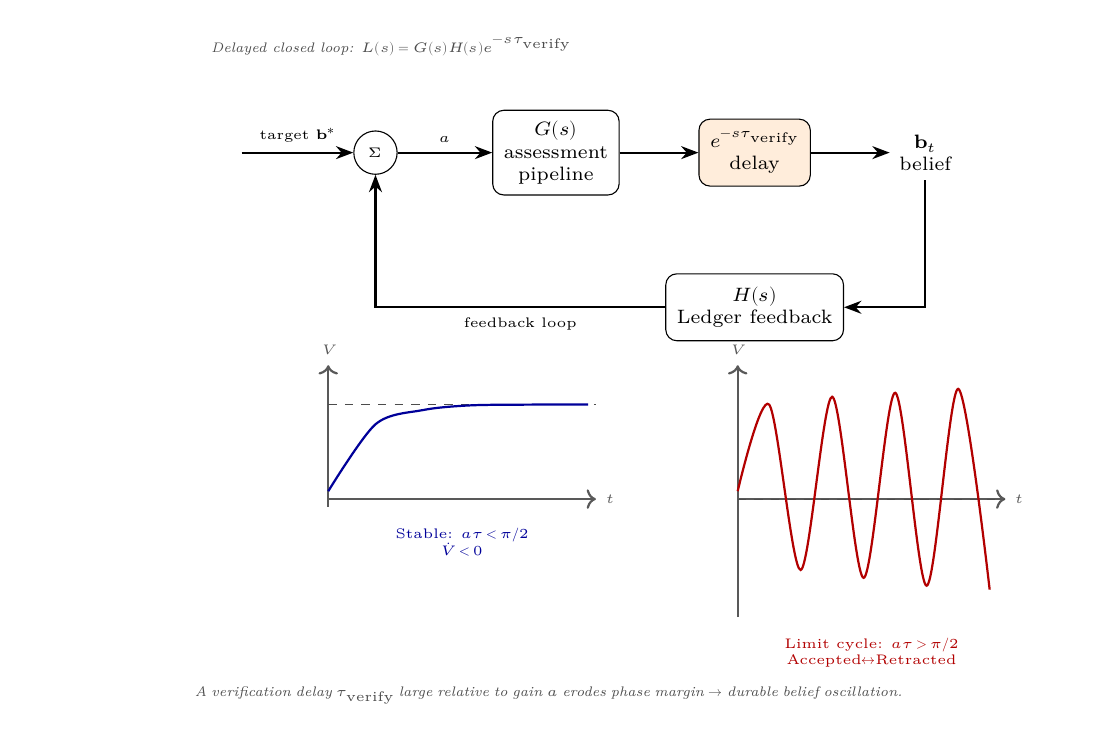
\begin{tikzpicture}[
  box/.style={rectangle, draw, rounded corners, align=center, font=\scriptsize, inner sep=4pt, minimum height=0.85cm},
  sum/.style={circle, draw, inner sep=1pt, minimum size=0.55cm, font=\tiny},
  arrow/.style={-{Stealth[length=2.2mm]}, thick},
  label/.style={font=\tiny\itshape, text=gray!60!black},
  ax/.style={->, gray!70!black, thick},
]

% === BLOCK DIAGRAM (top) ===
\node[sum] (sj) at (0,3) {$\Sigma$};
\node[box, right=1.2cm of sj] (G) {$G(s)$\\assessment\\pipeline};
\node[box, right=1.0cm of G, fill=orange!14] (delay) {$e^{-s\tau_{\mathrm{verify}}}$\\delay};
\node[right=1.0cm of delay, align=center, font=\scriptsize] (out) {$\mathbf{b}_t$\\belief};
\node[box, below=1.1cm of delay] (H) {$H(s)$\\Ledger feedback};

\draw[arrow] (-1.7,3) -- node[above,font=\tiny]{target $\mathbf{b}^*$} (sj);
\draw[arrow] (sj) -- node[above,font=\tiny]{$a$} (G);
\draw[arrow] (G) -- (delay);
\draw[arrow] (delay) -- (out);
\draw[arrow] (out.south) |- (H.east);
\draw[arrow] (H.west) -| node[pos=0.25,below,font=\tiny]{feedback loop} (sj.south);

\node[label, align=left] at (0.2,4.35) {Delayed closed loop: $L(s)=G(s)H(s)e^{-s\tau_{\mathrm{verify}}}$};

% === STABLE STEP RESPONSE ===
\begin{scope}[shift={(-0.6,-1.4)}]
  \draw[ax] (0,0) -- (3.4,0) node[right,font=\tiny]{$t$};
  \draw[ax] (0,-0.1) -- (0,1.7) node[above,font=\tiny]{$V$};
  \draw[dashed, gray!60!black] (0,1.2) -- (3.4,1.2);
  \draw[thick, blue!60!black] plot[smooth] coordinates {(0,0.1)(0.6,0.95)(1.2,1.13)(1.8,1.19)(2.6,1.2)(3.3,1.2)};
  \node[font=\tiny, align=center, text=blue!60!black] at (1.7,-0.55) {Stable: $a\tau<\pi/2$\\$\dot V<0$};
\end{scope}

% === OSCILLATORY STEP RESPONSE ===
\begin{scope}[shift={(4.6,-1.4)}]
  \draw[ax] (0,0) -- (3.4,0) node[right,font=\tiny]{$t$};
  \draw[ax] (0,-1.5) -- (0,1.7) node[above,font=\tiny]{$V$};
  \draw[dashed, gray!60!black] (0,0) -- (3.4,0);
  \draw[thick, red!70!black] plot[smooth] coordinates {(0,0.1)(0.4,1.2)(0.8,-0.9)(1.2,1.3)(1.6,-1.0)(2.0,1.35)(2.4,-1.1)(2.8,1.4)(3.2,-1.15)};
  \node[font=\tiny, align=center, text=red!70!black] at (1.7,-1.95) {Limit cycle: $a\tau>\pi/2$\\Accepted$\leftrightarrow$Retracted};
\end{scope}

\node[label, align=center, text width=13cm] at (2.2,-3.9)
  {A verification delay $\tau_{\mathrm{verify}}$ large relative to gain $a$ erodes phase margin $\rightarrow$ durable belief oscillation.};
\end{tikzpicture}
\end{document}
